%%%%%%%%%%%%%%%%%%%%%%%%%%%%%%%%%%%%%%%%%
% Daily Laboratory Book
% LaTeX Template
%
% This template has been downloaded from:
% http://www.latextemplates.com
%
% Original author:
% Frank Kuster (http://www.ctan.org/tex-archive/macros/latex/contrib/labbook/)
%
% Important note:
% This template requires the labbook.cls file to be in the same directory as the
% .tex file. The labbook.cls file provides the necessary structure to create the
% lab book.
%
% The \lipsum[#] commands throughout this template generate dummy text
% to fill the template out. These commands should all be removed when 
% writing lab book content.
%
% HOW TO USE THIS TEMPLATE 
% Each day in the lab consists of three main things:
%
% 1. LABDAY: The first thing to put is the \labday{} command with a date in 
% curly brackets, this will make a new page and put the date in big letters 
% at the top.
%
% 2. EXPERIMENT: Next you need to specify what experiment(s) you are 
% working on with an \experiment{} command with the experiment shorthand 
% in the curly brackets. The experiment shorthand is defined in the 
% 'DEFINITION OF EXPERIMENTS' section below, this means you can 
% say \experiment{pcr} and the actual text written to the PDF will be what 
% you set the 'pcr' experiment to be. If the experiment is a one off, you can 
% just write it in the bracket without creating a shorthand. Note: if you don't 
% want to have an experiment, just leave this out and it won't be printed.
%
% 3. CONTENT: Following the experiment is the content, i.e. what progress 
% you made on the experiment that day.
%
%%%%%%%%%%%%%%%%%%%%%%%%%%%%%%%%%%%%%%%%%

%---------------------------------------------------------------------
%	PACKAGES AND OTHER DOCUMENT CONFIGURATIONS
%----------------------------------------------------------------------

\documentclass[idxtotoc,hyperref,openany,oneside]{labbook} % 'openany' here removes the gap page between days, erase it to restore this gap; 'oneside' can also be added to remove the shift that odd pages have to the right for easier reading

\usepackage[ 
  backref=page,
  pdfpagelabels=true,
  plainpages=false,
  colorlinks=true,
  bookmarks=true,
  pdfview=FitB]{hyperref} % Required for the hyperlinks within the PDF
  
\usepackage{booktabs} % Required for the top and bottom rules in the table
\usepackage{float} % Required for specifying the exact location of a figure or table
\usepackage{graphicx} % Required for including images
\usepackage{lipsum} % Used for inserting dummy 'Lorem ipsum' text into the template
\usepackage{mathrsfs}
\usepackage{amsmath}
\usepackage{soul}

\newcommand{\HRule}{\rule{\linewidth}{0.5mm}} % Command to make the lines in the title page
\setlength\parindent{0pt} % Removes all indentation from paragraphs

\usepackage{enumitem,amssymb}
\newlist{todolist}{itemize}{2}
\setlist[todolist]{label=$\square$}
\usepackage{pifont}
\newcommand{\cmark}{\ding{51}}%
\newcommand{\xmark}{\ding{55}}%
\newcommand{\done}{\rlap{$\square$}{\raisebox{2pt}{\large\hspace{1pt}\cmark}}%
  \hspace{-2.5pt}}
\newcommand{\wontfix}{\rlap{$\square$}{\large\hspace{1pt}\xmark}}
\newcommand{\tss}{\textsuperscript}
\newcommand{\tsbs}{\textsubscript}

%---------------------------------------------------------------------
%	DEFINITION OF EXPERIMENTS
%---------------------------------------------------------------------

\newexperiment{Notes}{Experiment Notes}
\newexperiment{Stock}{Stock creation}
\newexperiment{Cycle1Prep}{Preparation for Cycle 1}
\newexperiment{Cycle1}{Cycle 1 experiment}
\newexperiment{Cycle1_Counting}{Counting for Cycle 1 experiment}
\newexperiment{table1}{Isotopes we are looking for}
%\newexperiment{shorthand}{Description of the experiment}

%----------------------------------------------------------------------
\begin{document}

%----------------------------------------------------------------------
%	TITLE PAGE
%-----------------------------------------------------------------------

\frontmatter % Use Roman numerals for page numbers
\title{
\begin{center}
\HRule \\[0.4cm]
{\Huge \bfseries Laboratory Journal }\\[0.4cm] % Degree
\HRule \\[1.5cm]
\end{center}
}
\author{\Huge Paul Mendoza \\ \\ \LARGE paul.m.mendoza@gmail.com \\[2cm]}
\date{This notebook begins 6 October 2016} 
\maketitle

\tableofcontents

\mainmatter 

%------------------------------------------------------------------------
%	LAB BOOK CONTENTS
%------------------------------------------------------------------------




%------------------------------------------------------------------------
%	LAB BOOK day
%-----------------------------------------------------------------------

\labday{Thursday, 6 October 2016\\ 8:30am - 11:00 am\\ 1:30pm - 3:30pm}

\experiment{table1}
\begin{itemize}
\item{Decay Monitors}
  \begin{itemize}
  \item{\tss{137}Cs/\tss{133}Cs}
  \end{itemize}
\item{Burnup Monitor}
  \begin{itemize}
  \item{(\tss{154}Eu/\tss{153}Eu) [\tss{155}Eu]}
  \end{itemize}
\item{Reactor type monitors}
  \begin{itemize}
  \item{(\tss{134}Cs/\tss{137}Cs)}
  \item{(\tss{150}Sm/\tss{149}Sm)}
  \item{(\tss{242}Pu/\tss{239}Pu)}
  \item{(\tss{135}Cs/\tss{137}Cs)}
  \item{(\tss{136}Ba/\tss{138}Ba)}
  \end{itemize}
\item{Isotope Solve list}
\end{itemize}

\begin{table}[H]
\begin{center}
\begin{tabular}{l l l}
\toprule
\tss{133}Cs & \tss{136}Ba & \tss{153}Eu\\ 
\tss{134}Cs & \tss{138}Ba & \tss{154}Eu\\
\tss{135}Cs & \tss{149}Sm & \tss{239}Pu\\
\tss{137}Cs & \tss{150}Sm & \tss{242}Pu\\
\bottomrule
\end{tabular}
\caption{Isotope solve list.}
\end{center}
\end{table}  

\experiment{Notes}

\begin{itemize}
\item{Project Number: 504370-0001}
\item{Files on computer saved in C:/Paul\_Mendoza}
\item{Stock HNO\tsbs{3}: Assuming Temp=24.8+/-3 $\rightarrow\boxed{Stock\ HNO_3}$}
  \begin{itemize}
  \item{Molarity : 15.35+/-0.13}
  \item{pH: -1.186+/-0.004}
  \item{Molality: 35.3+/-0.8}
  \item{Wt Concentration: 69.0+/-0.5}
  \item{Molar Mass: 63.0130+/-0.0012}
  \item{Density: 1.402+/-0.006}
  \end{itemize}
\item{Stock Iron Sulfamate $Fe(NH_2SO_3)_2$ $\rightarrow\boxed{Stock\ Fe(II)}$}
  \begin{itemize}
  \item{Molarity : 2.302+/-0.009}
  \item{Molality : 2.717+/-0.006}
  \item{Wt Concentration : 40.26+/-0.05}
  \item{Molar Mass : 248.022+/-0.017}
  \item{Density: 1.418+/-0.005}
  \end{itemize}
\end{itemize}

\experiment{Stock} % 

\begin{itemize}
\item{Get stock solution from Troy room 18A, store near rad waste}
\item{Grab 1000$\mu$l pipett from glovebox}
\item{Decontaminate with radic - dump waste into glass aq rad outside glove box}
\item{Practice pipetting 500$\mu$l to glass vial - setting 503 $\mu$l
  gives 500 $\mu$l}
\item{Class/lunch Break}
\item{Get alpha detector from Dr. Marianno}
\item{Set up laboratory notebook}
\item{Calculation}
  To do calculation to determine the volumes needed for a final
  concentration of a particular volume, knowing the initial
  concentrations
  \begin{align*}
    V_2&=\frac{b_2-\frac{M_1b_1}{A}}{M_2-\frac{M_1}{A}}\\
    V_1&=\frac{b-BV_2}{A}
  \end{align*}
  Where:
  \begin{align*}
    A&=(1-wt\%_1)\rho_1\\
    B&=(1-wt\%_2)\rho_2\\
    b_1&=(1-wt\%_3)V_3\rho_3\\
    b_2&=M_3V_3
  \end{align*}
  With known Molarity and volume of a solution
  how much, and of what concentration
  do we need to combine with a second solution
  to get a final solution of known concentration
  and volume?
  \begin{align*}
    B&=(1-wt\%_3)V_3\rho_3-(1-wt\%_1)V_1\rho_!\\
    A&=M_3V_3-M_1V_1\\
    C&=\frac{B}{A}=\frac{(1-wt\%_2)\rho_2}{M_2}
  \end{align*}
  Need iterative solution, choose:
  \begin{align*}
    M_2&=\frac{M_3V_3-M_1V_1}{V_3-V_1}\\
    V_2&=V_3-V_1
  \end{align*}
  Use to determine molality $\rightarrow$ $wt\%_2$ $\rightarrow$
  $\rho_2$. Then compare to $C$, iterate around the solution to
  find answer so that $C=\frac{(1-wt\%_2)\rho_2)}{M_2}$.
\end{itemize}

%------------------------------------------------------------------------
%	LAB BOOK day
%-----------------------------------------------------------------------

\labday{Friday, 7 October 2016\\ 9:00am - 12:00 am\\ 1:00pm - 4:00pm}

\experiment{Stock} % 

\begin{todolist}
\item[\done]{Program calculation for creation of stock - some
results shown below}
\item[\done]{Prepare shielding for transfer for closet solution}
  \begin{itemize}
  \item{Clean off and move leaded shielding in rad area to
    countertop next to fumehood}
  \item{Add diaper paper on countertop, and on shielding incase
    of contamination}
  \item{Practice transfer}
  \end{itemize}
\item[\done]{-}
\end{todolist}
\begin{center}
    0.149+/-0.011 ml of 15.43+/-0.06 M HNO\tsbs{3} $\boxed{Stock\ HNO_3}$\\
    +\\
    1.91+/-0.08  ml of 0.0+/-0 M solution $\boxed{DI\ Water}$\\
    = \\
    2.048+/-0.026 ml of 1.12+/-0.08 M HNO\tsbs{3}
  solution $\boxed{\rightarrow Stock}$ (glass container)
\end{center}
\begin{todolist}
\item[\done]{-}
\end{todolist}
\begin{center}
Combine 0.500+/-0.005 ml of 15.43+/-0.06 M HNO\tsbs{3}
solution $\boxed{closet}$\\
+\\
2.048+/-0.026 ml of 1.12+/-0.08 M HNO\tsbs{3} solution
$\boxed{Stock}$
\\
=\\
2.500+/-0.025 ml of 4.00+/-0.05 M HNO\tsbs{3} solution.
$\boxed{\rightarrow Stock}$
\end{center}

\begin{todolist}
\item[\done]{Lock $\boxed{Stock}$ in glovebox}
\item[\done]{Put Source back in rad closet}
\item[\done]{Clean up contamination added to pipette tip from transfer (for some reason, the contamination was added to the inside of the pipette itself, the tips used don't have the block, but still, none of the solution should have traveled up the shaft}
\item[\done]{Dispose of diaper paper laid down for transfer (where the glass bottle was set down which contained closet solution, there was contamination (the outside of the bottle of the closet solution is contaminated)}
\item[\done]{Move shielding back to where it was}
\end{todolist}

\experiment{Cycle1Prep}
\begin{todolist}
\item[\done]{Count calibration standard Eu-152 in HPGe 3 hours 22 minutes at furtherest position from detector (26 cm)}
  \begin{itemize}
  \item{Source 1577-22}
  \item{497.0 nCi}
  \item{Assy Date: 15 Feb 12}
  \item{1.00568g}
  \end{itemize}
\item[\done]{Create Eu-152 Excel Counting sheet template for standards}
\item[\done]{Set up ROI (region of interest) file for Eu-152}
\item[\done]{Start background count and done for the day}
  \begin{itemize}
  \item{Count lasted for 12 hours}
  \end{itemize}
\end{todolist}

%------------------------------------------------------------------------
%	LAB BOOK day
%-----------------------------------------------------------------------

\labday{Saturday, 8 October 2016\\ 10:00am - 2:00 pm}

\experiment{Cycle1Prep}

\begin{todolist}
\item[\done]{Finish background count, lasted 12 hours}
\item[\done]{Remove 0.3 ml from $\boxed{Stock}$ transfer to $\boxed{1}$
  for counting}
  \begin{itemize}
  \item{$\boxed{1}$ is a smaller tube, which will fit into a larger
    centrifuge tube for, well, centrifuging}
  \item{$\boxed{1}$ tube cannot fit into centrifuge tube with white
    push cap (pushes on outside of tube),
    white push cap is necessary when votex mixing, so a blue push cap
    (pushes on inside of tube), was put on for counting, these smaller
    tubes will have to have two caps following them around, I can't
    wait till the second cycle when the bigger tubes will be used}
  \item{Note for why smaller tubes are being used: when pipetting the
    smaller volume of 0.3 ml for aq/o phase separation it is much
    easier to have the smaller diameter tubes}
  \item{Stock was removed from glovebox, and after was put into the safe}
  \end{itemize}
\item[\done]{Count $\boxed{1}$ for 1 hour and 24 minutes}
\item[\done]{Fix density calculation in code, was slightly wrong before,
  this means $\boxed{Stock}$ and $\boxed{1}$ are slightly different
  from what they should be, but within error}
\item[\done]{Calculation for creation of Fe(II) solution (next page)}
\end{todolist}
\clearpage
\begin{center}
  $V_1$ ml of $M_{1,Fe}$ Fe(II) in $M_{1,HNO_3}$ HNO\tsbs{3}\\
  $+$\\
  $V_2$ ml of $M_{2,Fe}$ Fe(II) in $M_{2,HNO_3}$ HNO\tsbs{3}\\
  =\\
$V_3$ ml of $M_{3,Fe}$ Fe(II) in $M_{3,HNO_3}$ HNO\tsbs{3}.
\end{center}

The knowns are: \\
$M_{1,Fe}=2.302$, $\rho_1=1.418$, $M_{1,HNO_3}=0$ (Fe Stock soltuion)\\
$M_{2,Fe}=0$,$\rho_2=\rho_{HNO_3}(M_{2,HNO_3})$ \\
$V_3=4$ ml, $M_{3,Fe}=0.024$, $M_{3,HNO_3}=4$, $\rho_3=\rho_{HNO_3}(4M)$\\~\\

Mols of Fe(II) constant: $V_1=\frac{M_{3,Fe}V_3}{M_{1,Fe}}=0.042$\\
Mols of HNO\tsbs{3} constant: $V_2=\frac{V_3M_{3,HNO_3}}{M_{2,HNO_3}}$\\
Mass Constant: $V_2=\frac{V_3\rho_3-V_1\rho_1}{\rho_2}$\\~\\

Combine last two equations:$M_{2,HNO_3}-
\frac{V_3M_{3,HNO_3}\rho_2}{V_3\rho_3-V_1\rho_1}=0$\\~\\
Solve iteratively (where $M_{2,HNO_3}$ determines $\rho_2$)
with first guess of:
$M_{2,HNO_3}=\frac{M_{3,HNO_3}V_3}{V_2}$



%------------------------------------------------------------------------
%	LAB BOOK day
%-----------------------------------------------------------------------

\labday{Sunday, 9 October 2016\\ 7:30 pm - 11:30 pm}

\experiment{Cycle1Prep}

\begin{todolist}
\item[\done]{Prepare for multi contact extraction and back extraction exp}
  \begin{itemize}
  \item{Make solution of 30 vol.\% TBP with kerosene}
  \item{Make 40 ml of solution 4.06 M HNO\tsbs{3} solution, }
  \item{Transfer two smaller vials (one for TBP phase), one for
    Fe phase, with two different lids into glovebox (with
  a larger vial to hold them in the centrifuge)}
  \item{Transfer two smaller vials with centrifuge vials for
    centrifuging, keep one with water 0.3 ml, and TBP mix 0.32 ml
    $\boxed{Vial\ 1\ Budd}$, and
    the second with 1.2 ml of TBP mix and 1.25 ml water
    $\boxed{Vial\ 2\ Budd}$}
  \item{Transfer $\boxed{Stock}$ and $\boxed{1}$ to glovebox}
  \item{Transfer another vial to hold the Fe solution}
  \item{Make sure tweezers are in glovebox (they are) - to remove smaller
    vials from centrifuge tubes}
  \item{Transfer slightly contaminated pipette to glovebox}
  \item{All above vials that would contain solution were rinsed
    with whatever they would hold for approximately 3 minutes}
  \end{itemize}
\end{todolist}

\begin{todolist}
\item[\done]{-}
\end{todolist}
\begin{center}
15+/-0.15 ml of TBP $\boxed{Stock\ TBP}$\\
+\\
35+/-0.35 ml of kerosene $\boxed{Stock\ kerosene}$\\
=\\
50+/-0.5 ml of 30 vol.\% TBP.
$\boxed{\rightarrow TBP}$
\end{center}

\begin{todolist}
\item[\done]{-}
\end{todolist}
\begin{center}
10.579+/-0.011 ml of 15.35+/-0.13 M HNO\tsbs{3} $\boxed{Stock\ HNO_3}$\\
+\\
30.355+/-0.030 ml of 0.0+/-0 M HNO\tsbs{3} solution $\boxed{DI\ Water}$\\
=\\
39.94+/-0.14 ml of 4.07+/-0.04 M HNO\tsbs{3} solution
$\boxed{\rightarrow Fe\ Prep}$
\end{center}

To create an Fe solution for a back extraction, $\boxed{Fe\ Prep}$ should be
combined in the following manner (Small portions created because this
solution has a short half life with larger concentrations of $HNO_3$).

\begin{todolist}
\item{-}
\end{todolist}
\begin{center}
0.0417+/-0.0018 ml of 2.302+/-0.009 M Fe(II) in 0.0+/-0 M HNO\tsbs{3} $\boxed{Stock\ Fe(II)}$\\
+\\
3.941+/-0.027 ml of 0.0+/-0 M Fe(II) in 4.06+/-0.05 M HNO\tsbs{3} solution $\boxed{Fe\ Prep}$\\
+\\
4.000+/-0.020 ml of 0.0240+/-0.0010 M Fe(II) in 4.00+/-0.05 M HNO\tsbs{3} solution $\boxed{\rightarrow Bk\ Ex\ Solution}$.
\end{center}

\begin{todolist}
\item[\done]{Add Sodium Nitrite to $\boxed{1}$, it will sit overnight,
but it doesn't have to}
  \begin{itemize}
  \item{Dropped $\boxed{1}$, solution probably contaminated blue lid
    (crap), centrifuged on 1000 rpm for 2 minutes}
  \end{itemize}
\end{todolist}


%------------------------------------------------------------------------
%	LAB BOOK day
%-----------------------------------------------------------------------

\labday{Monday, 10 October 2016\\ 12:30 pm - 4:30 pm}

\experiment{Cycle1}
\begin{todolist}
\item[\done]{First contact - Extraction}
  \begin{itemize}
  \item{Add 0.32 ml $\boxed{TBP}$ to $\boxed{1}$}
  \item{Shake on Pulse Mode of 15 minutes on vortex mixer}
  \item{Change of plans (This occured while sample settled for
       a bit while changes were implemented)}
    \begin{itemize}
    \item{Put smaller tubes directly into centrifuge - so we do not
      have to switch caps so often}
    \item{Pulled out $\boxed{Vial\ 1\ Budd}$ and $\boxed{Vial\ 2\ Budd}$
      Pulled out of glovebox the smaller tubes,
      changed their caps, labeled them, put back into
      glovebox (5-10 minutes)}
    \end{itemize}
  \item{Centrifuge 1000 rpm for 10 minutes}
  \item{Attempted to pull out 0.30 ml of TBP phase}
    \begin{itemize}
    \item{Utter Failure}
    \item{Utter Failure again}
    \item{Utter failure...difficult to pull out 0.3 ml and keep
    phases separate}
    \end{itemize}
  \item{Added 1.08 ml $\boxed{TBP}$ to $\boxed{1}$ (for 0.2 ml buffer)}
    \begin{itemize}
    \item{All extractions at once (different from original exp)}
      \begin{align*}
        p=\frac{1}{1+\frac{1}{D}\frac{V_{aq}}{V_o}}
      \end{align*}
    \item{$V_o$ increased by fourfold}
    \item{Pipette slipped to 538 (instead of 540 $\rightarrow$ 0.4\%
      increase in error)}
    \end{itemize}
  \item{Vortex mix for 15 minutes on pulse mode}
  \item{Centrifuge 1000 cpm for 10 minutes}
  \item{Remove 1000 ml top phase (TBP), then remove
    another 200 ml of top phase (TBP) $\boxed{\rightarrow 2}$}
  \end{itemize}
\item[\done]{Creation of $\boxed{Bk\ Ex\ Solution}$}
\end{todolist}
\begin{center}
0.0417+/-0.0018 ml of 2.302+/-0.009 M Fe(II) in 0.0+/-0 M HNO\tsbs{3} $\boxed{Stock\ Fe(II)}$\\
+\\
3.941+/-0.027 ml of 0.0+/-0 M Fe(II) in 4.06+/-0.05 M HNO\tsbs{3} solution $\boxed{Fe\ Prep}$\\
+\\
4.000+/-0.020 ml of 0.0240+/-0.0010 M Fe(II) in 4.00+/-0.05 M HNO\tsbs{3} solution $\boxed{\rightarrow Bk\ Ex\ Solution}$.
\end{center}
\begin{todolist}
\item[\done]{Back Extraction - First Contact}
  \begin{itemize}
  \item{Add 1.4 $\boxed{Bk\ Ex\ Solution}$ to $\boxed{2}$}
  \item{Shake pulse mode for 15 minutes}
  \item{Remove 1.2 ml of bottom phase (Fe(II)) $\boxed{\rightarrow 3}$}
    \begin{itemize}
    \item{Lost two drops}
    \item{While placing vial into centrifuge, cap shot off,
      spraying solution everywhere...great}
    \end{itemize}
  \end{itemize}
\item[\done]{Back Extraction - Second Contact}
  \begin{itemize}
  \item{Add 1.4 $\boxed{Bk\ Ex\ Solution}$ to $\boxed{2}$}
  \item{Shake pulse mode for 15 minutes}
  \item{Remove 1.2 ml of bottom phase (Fe(II)) $\boxed{\rightarrow 3}$}
  \end{itemize}
\item[\done]{Back Extraction - Third Contact}
  \begin{itemize}
  \item{Add 1.4 $\boxed{Bk\ Ex\ Solution}$ to $\boxed{2}$}
  \item{Shake pulse mode for 15 minutes}
  \item{Remove 1.2 ml of bottom phase (Fe(II)) $\boxed{\rightarrow 3}$}
  \end{itemize}
\end{todolist}
\vspace{5mm}
This experiment had sputtering of pipette at certain times.

\experiment{Cycle1_Counting}
\begin{todolist}
\item[\done]{Counted waste $\boxed{1}$, containing 0.3
  ml of $\boxed{Stock}$ and 0.2 ml $\boxed{TBP}$, on HPGe,
  for 12 hours (left for the night)}
\end{todolist}

%------------------------------------------------------------------------
%	LAB BOOK day
%-----------------------------------------------------------------------

\labday{Tuesday, 11 October 2016\\ 10:30 pm - 1:00 am}

\experiment{Cycle1_Counting}
There are 6 things to count.
\begin{todolist}
\item[\done]{Initial solution $\boxed{1}$ - 23 cm away, 0.3 ml HNO\tsbs{3}}
\item[\done]{Waste $\boxed{1}$ - 23 cm away, 0.3 ml HNO\tsbs{3} 0.2 ml TBP}
\item[\done]{Create 4 M HNO\tsbs{3} solution store in fume hood}
\end{todolist}
\begin{center}
2.6056+/-0.0026 ml of 15.35+/-0.13 M HNO\tsbs{3} solution $\boxed{Stock\ HNO_3}$\\
+\\
7.625+/-0.008 ml of 0.0+/-0 M HNO\tsbs{3} solution $\boxed{DI}$\\
+\\
9.985+/-0.035 ml of 4.01+/-0.04 M HNO\tsbs{3} solution $\boxed{\rightarrow 4\ M\ HNO_3}$.
\end{center}
\begin{todolist}
\item[\done]{Pull out 0.2 from bottom of $\boxed{1}$ (HNO\tsbs{3}),
  dillute to 0.3 ml with $\boxed{4\ M\ HNO_3}$ $\boxed{\rightarrow 1W}$}
  \begin{itemize}
  \item{Count on HPGe $\sim$ 1 hour}
  \end{itemize}
\item[\done]{Pull out 0.3 ml from $\boxed{3}$ to count
  $\boxed{\rightarrow 3P}$ (product)}
  \begin{itemize}
  \item{Start Count on HPGe 4 hours (left overnight)}
  \end{itemize}
\item[\done]{Pull out 0.3 ml from top of $\boxed{2}$ (TBP), to count
       $\boxed{\rightarrow 2W}$ (Waste)}
\item{\st{Pull out 0.7 ml from top of $\boxed{2}$ (TBP)
  $\boxed{\rightarrow 2W2}$, then count $\boxed{2}$ - which should
    have 0.3 ml, 0.1 ml of TBP, and 0.2 ml of HNO}\tsbs{3}}
  \begin{itemize}
  \item{Coult not pull out all 0.7, but only 0.6}
  \end{itemize}
\item[\done]{Pull out 0.6 ml from top of $\boxed{2}$ (TBP)
  $\boxed{\rightarrow 2W2}$, should have 0.4 ml, 0.2 ml of TBP,
  and 0.2 ml of HNO\tsbs{3}}
\end{todolist}


\begin{figure}[H] % Example of including images
\begin{center}
  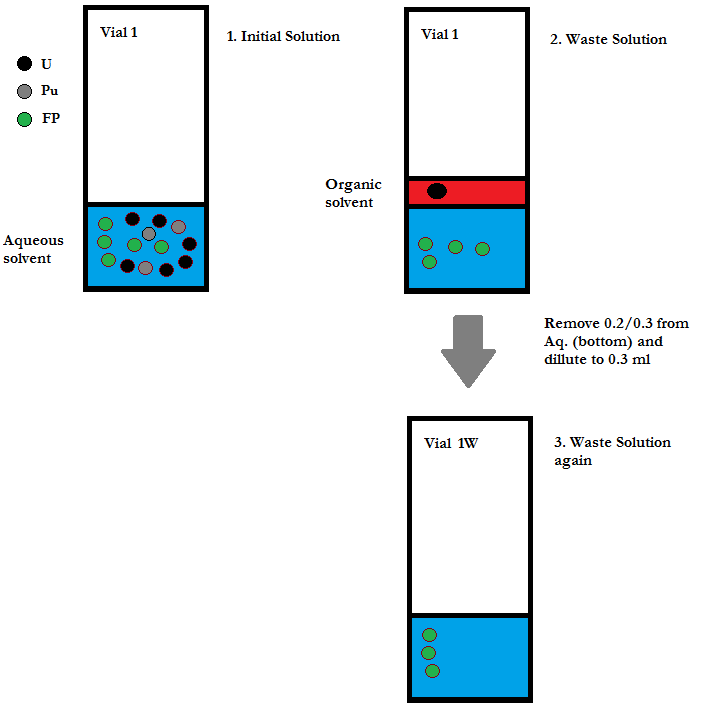
\includegraphics[width=0.6\linewidth]
                  {Figures/Extraction_Cycle_1_First_3_Counts}
\end{center}
\caption{First Three Counts}
\label{fig:example1}
\end{figure}

\begin{figure}[H] % Example of including images
\begin{center}
  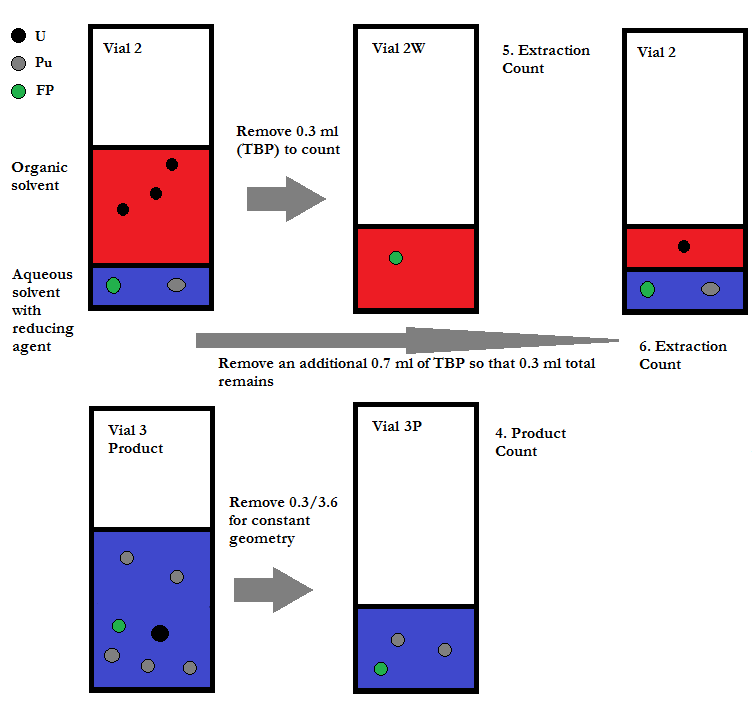
\includegraphics[width=0.6\linewidth]
                  {Figures/Back_Extraction_Cycle_1_Last_3_Counts}
\end{center}
\caption{Second Three Counts}
\label{fig:example2}
\end{figure}



%----------------------------------------------------------------------
%	Examples
%-----------------------------------------------------------------------
%---------------------------------------
% Blank template to use for new days:
%---------------------------------------
%\labday{Day, Date Month Year}
%\experiment{}
%Text

%---------------------------------------
% To do list
%---------------------------------------
%% \begin{todolist}
%% \item[\wontfix]{profit}
%% \item[\done]{This is done}
%% \item{This is not done}
%% \end{todolist}

%---------------------------------------
% Vial Step
%---------------------------------------
%% \begin{todolist}
%% \item{-}
%% \end{todolist}
%% \begin{center}
%% Vial 1\\
%% +\\
%% Vial 2\\
%% =\\
%% Final Vial
%% \end{center}

%% \labday{Example} % We don't want a date here so we make the labday blank

%% \begin{center}
%% \HRule \\[0.4cm]
%% {\huge \textbf{Examples}}\\[0.4cm] % Heading
%% \HRule \\[1.5cm]
%% \end{center}

%% %-----------------------------------------------------------------------
%% %	Formulae
%% %-----------------------------------------------------------------------
%% \huge \textbf{Formulae} \\ \\

%% \normalsize \textbf{Formula 1 - Pythagorean theorem}\\ \\
%% $a^2 + b^2 = c^2$\\ \\

%% %--------------------------------------------------------------
%% %	Citation
%% %--------------------------------------------------------------

%% Citation test \cite{Tatro2013}.

%% %--------------------------------------------------------------
%% %	Figure
%% %--------------------------------------------------------------

%% \begin{figure}[H] % Example of including images
%% \begin{center}
%% 
\includegraphics[width=0.5\linewidth]{Figures/example_figure}
%% \end{center}
%% \caption{Example figure.}
%% \label{fig:example_figure}
%% \end{figure}

%% %--------------------------------------------------------------
%% %	Table
%% %--------------------------------------------------------------

%% \experiment{table}

%% \begin{table}[H]
%% \begin{tabular}{l l l}
%% \toprule
%% \textbf{Groups} & \textbf{Treatment X} & \textbf{Treatment Y} \\
%% \toprule
%% 1 & 0.2 & 0.8\\
%% 2 & 0.17 & 0.7\\
%% 3 & 0.24 & 0.75\\
%% 4 & 0.68 & 0.3\\
%% \bottomrule
%% \end{tabular}
%% \caption{The effects of treatments X and Y on the four groups studied.}
%% \label{tab:treatments_xy}
%% \end{table}

%% Table \ref{tab:treatments_xy} shows that groups 1-3 reacted similarly to the two treatments but group 4 showed a reversed reaction.

%% %------------------------------------------------------------
%% %	Bibliography
%% %------------------------------------------------------------
%% \bibliography{references} 
%% \bibliographystyle{plain} 

\end{document}

